\section{Struttura del Progetto}
Il progetto è incluso in una cartella contenente anche il software di ricerca di RFD, tutto il codice sviluppato è contenuto nella sottocartella query{\_}rewriter
\begin{figure}[H]
    \centering
    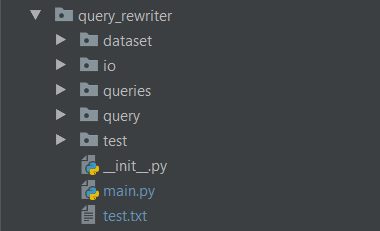
\includegraphics{struct_project.png}
    \caption{Struttura del Progetto}
    \label{fig:struct_project}
\end{figure}

\subsection{Package Dataset}
Il package Dataset include una serie di Dataset in formato $csv$ ed una cartella contente le rispettive liste di RFD già precalcolate. 
I Dataset inclusi nel progetto sono:
\begin{itemize}[noitemsep]
\let\labelitemi\labelitemii
    \item cars.csv
    \item cars2.csv
    \item cars{\_}db.csv
    \item cora.csv
    \item crawled-tweets.csv
    \item dataset.csv
    \item dataset{\_}string.csv
    \item dataset{\_}string2.csv
    \item echocardiogram.csv
    \item iris.csv
    \item restaurant
\end{itemize}

Sono state già calcolate le seguenti liste di RFD:
\begin{itemize}[noitemsep]
\let\labelitemi\labelitemii
    \item cars{\_}db{\_}rfds.csv
    \item cars{\_}rfds.csv
    \item cora{\_}rfds.csv
    \item dataset{\_}rdfs.csv
    \item dataset{\_}strng{\_}rfds.csv
\end{itemize}


La maggior parte dei Dataset sono in formato numerico, ma ne sono presenti alcuni che possiedono attributi sia in formato numerico che di tipo stringa

\subsection{Package io}
In questo package sono contenuti diversi moduli divisi in baso al loro scopo. Vi sono due sottocartelle che raggruppano il tutto.
Il contenuto nella sotto-cartella csv comprende:
\begin{itemize}[noitemsep]
\let\labelitemi\labelitemii
    \item csv{\_}parser.py
    \item io.py
\end{itemize}

\paragraph{csv{\_}parser.py}
Questo modulo contiene la classe CSV Parser che si occupa di prendere i dati dai file CSV e salvarli in un Dataframe, il tutto viene fatto nel metodo init(\ldots).
\begin{listing}[H]
\begin{minted}[frame=lines,linenos]{python}
class CSVParser:
    def __init__(self, csv_path: str):
        self.path = csv_path
        self.delimiter = self.__guess_delimiter()
        self.data_frame = pd.read_csv(self.path, 
                                delimiter=self.delimiter)
        self.rows_count, self.columns_count = self.data_frame.shape
        self.header = list(self.data_frame)
\end{minted}
\caption{Class CSVParser}
\label{Code:1}
\end{listing}
L'operazione vera e propria di $parsing$ e $loading$ dei dati viene delegata al Framework Pandas, richiamando il metodo alla riga 5.
Le variabili di questa classe sono:
\begin{itemize}[noitemsep]
\let\labelitemi\labelitemii
    \item path:[str] Contiene il path del file CSV
    \item delimiter:Contiene il carattere di separazione
    \item data{\_}frame:[Pandas Dataframe] Contiene i dati del file CSV letto
    \item rows{\_}count:[int]contiene il numero di righe contenute nel file CSV
    \item column{\_}count:[int]contiene il numero di colonne contenute nel file CSV
    \item header:[list] contiene una lista di valori che fungono da header, questi valori sono specificati nella prima riga del file csv
\end{itemize}
L'unico argomento da passare al costruttore è il path del file, tutti gli altri dati vengono calcolati. 
All'interno del costruttore è presente una chiamata al metodo {\_\_}guess{\_}delimiter:

\begin{listing}[H]
\begin{minted}[frame=lines,linenos]{python}
    def __guess_delimiter(self):
\end{minted}
\caption{Guess delimiter}
\label{Code:2}
\end{listing}

Questo metodo ha il compito di indovinare il carattere di separazione leggendo il file.

\paragraph{io.py}
Questo modulo contiene la classe CSVInputOutput la quale si occupa di importare/esportare una Pandas.Dataframe da/in un file CSV
\begin{listing}[H]
\begin{minted}[,frame=lines,linenos]{python}
    class CSVInputOutput:
\end{minted}
\caption{CSVInputOutput}
\label{Code:3}
\end{listing}
Le variabili di questa classe sono:
\begin{itemize}[noitemsep]
    \item sep:[str] campo contenente il simbolo di separazione utilizzato nei file CSV.
    \item na{\_}rep:[str] campo contenente il simbolo che rappresenta un dato mancante. 
    \item index:[boolean] flag che indica se si vuole stampare nel file csv gli indici di riga.
    \item encoding:[str] campo contente la codifica dei file input/output.
    \item date{\_}format:[str] campo contente il formato delle date.
\end{itemize}
Questa classe possiede due metodi.
Il primo è il metodo store
\begin{listing}[H]
\begin{minted}[frame=lines,linenos]{python}
    def store(self, df: pd.DataFrame, path: str):
\end{minted}
\caption{store method}
\label{Code:4}
\end{listing}
Questo metodo prende in input il path del del file in cui andare a salvare il DataFrame.

Il secondo è il metodo load:
\begin{listing}[H]
\begin{minted}[frame=lines,linenos]{python}
    def load(self, path: str) -> pd.DataFrame:
\end{minted}
\caption{load method}
\label{Code:5}
\end{listing}
Il metodo prende in input il path del file e delegando a Pandas Dataframe esegue il parsing e il loading.


La seconda sotto-cartella rfd contiene vari moduli inerenti alla manipolazione delle RFD:
\begin{itemize}[noitemsep]
\let\labelitemi\labelitemii
    \item rfd{\_}extractor.py
    \item store{\_}and{\_}load.py
\end{itemize}

\paragraph{rfd{\_}extractor.py}
Contiene la classe RFDExtractor che si occupa di estrarre le RFD da un dataset.
\begin{listing}[H]
\begin{minted}[frame=lines,linenos]{python}
class RFDExtractor:
    ...
    def __init__(self, args, debug_mode=False) -> None:
    ...
    def __str__(self) -> str:
    ...
    def extract_args(self, args):
    ...
    def extract_hss(self, cols_count, lhs, rhs):
    ...
    def extract_sep_n_header(self, c_sep, csv_file, has_header):
    ...
    def check_correctness(self, has_dt, hss, index_col):
    ...
    def usage(self):
    ...
    def print_human(self, rfd_data_frame: pd.DataFrame):
    ...
    def get_rfd_dictionary_list(self) -> list:
    ...
\end{minted}
\caption{RFDExtractor}
\label{Code:6}
\end{listing}

Non saranno fornite particolari informazioni su questa classe , in quanto essa fa parte del progetto riguardante la ricerca di RFD , per ulteriori informazioni si veda \cite{tesinaIA}

\paragraph{store{\_}and{\_}load.py}
È un modulo che ha funzione di wrapping per l'algoritmo di ricerca di RFD.
Contiene due metodi:
\begin{listing}[H]
\begin{minted}[frame=lines,linenos]{python}
def diff(list1: list, list2: list):
...
def search_rfds(csvPath,name_rfds_file):
\end{minted}
\caption{Metodi store{\_}load{\_}rfds}
\label{Code:7}
\end{listing}

IL primo metodo "diff" prende in input due liste, e restituisce una lista di elementi che sono presenti nella prima ma non nella seconda.

Il secondo metodo richiama l'algoritmo di Ricerca delle RFD \footnote{In questo caso non è semplice richiamo di una funzione, bensì vengono richiamati una serie di metodi, e mano a mano vengono effettuate delle elaborazioni sui dati} e crea un file contente una lista di RFD. Prende in input il path del file contenente il Dataset, e una stringa che contiene il nome del file che incapsula le RFD. 

\subsection{Package query}
Nel package query vi sono tre moduli, tutte e tre si occupano di svolgere operazioni riguardanti le interrogazioni al dataset.
I tre moduli sono:
\begin{itemize}[noitemsep]
\let\labelitemi\labelitemii
    \item relaxer.py
    \item slicer.py
\end{itemize}

\paragraph{relaxer.py}
Questo modulo contiene la classe QueryRelaxer, è una classe ausiliaria, contiene dei metodi statici che si occupano di rilassare la query rispetto ad una Relaxed Functional Dependency. La classe contiene i seguenti metodi:

\begin{listing}[H]
\begin{minted}[frame=lines,linenos]{python}
class QueryRelaxer:
    @staticmethod
    def drop_query_nan(rfds_df: pd.DataFrame, query: dict) 
                                            -> pd.DataFrame:
    ...
    @staticmethod
    def drop_query_rhs(rfds_df: pd.DataFrame, query: dict)
                                            -> pd.DataFrame:
    ...
    @staticmethod
    def sort_by_decresing_nan_incresing_threshold(rfds_df: 
                pd.DataFrame, query: dict) -> pd.DataFrame:
    ...
    @staticmethod
    def sort_by_increasing_threshold(rfds_df: pd.DataFrame,
        data_set: pd.DataFrame, query: dict) -> pd.DataFrame:
    ...
    @staticmethod
    def rfd_to_string(rfd: dict) -> str:
    ...
    @staticmethod
    def query_dict_to_expr(query: dict) -> str:
    ...
    @staticmethod
    def extend_query_ranges(query: dict, rfd: dict, 
            data_set: pd.DataFrame = None) -> dict:
    ...
    @staticmethod
    def similar_strings(source: str, data: pd.DataFrame,
                        col: str, threshold: int) -> list:
    ...
    @staticmethod
    def extract_value_lists(df: pd.DataFrame, columns: list):
    ...
\end{minted}
\caption{Classe Query Relaxer}
\label{Code:10}
\end{listing}

Il metodo drop{\_}query{\_}na(...) si occupa di eliminare tutte le RFD che possiedono valori NaN su attributi che sono contenuti anche nella query. Il metodo prende in input un pandas.Dataframe contenente la lista di RFD ed un dizionario contenente la query, restituisce un altro pandas.Dataframe.

Il metodo drop{\_}query{\_}rhs(...) si occupa di eliminare tutte le RFD che possiedono un attributo della query come parte RHS. Il metodo prende in input un pandas.Dataframe contenente la lista di RFD ed un dizionario contenente la query, restituisce un altro pandas.Dataframe.

Il metodo sort{\_}by{\_}decreasing{\_}nan{\_}incresing{\_}threshold(...), contiene un algoritmo di ordinamento. Il metodo prende in input un pandas.Dataframe ordina prima per numero di NaN presenti e poi per ordine crescente rispetto alla soglie, restituisce un pandas.Dataframe.

Il metodo sort{\_}by{\_}increasing{\_}threshold(...) , contiene un altro algoritmo di ordinamento, che è stato utilizzato solo nei test, dove è risultato poco producente. Il metodo prende in input un pandas.Dataframe e un dizionario contenente la query. Restitusce un altro pandas.Dataframe ordinato solo rispetto alle soglie degli attributi \footnote{In entrambi gli algoritmi di ordinamento vengono ordinate prima le soglie degli attributi contenuti nella query e poi in caso di valori uguali si ordina rispetto alle soglie degli altri attributi in LHS}.

il metodo rfd{\_}to{\_}string(...) svolge un ruolo alquanto semplice, si occupa di convertire il formato delle RFD in un formato stringa facilmente leggibile.

Questo metodo converte il dizionario nel formato stringa richiesto dal Dataframe di Pandas.
Qui è importante fare delle precisazioni dato che in  questa parte del codice vengono definite le condizioni che si possono applicare alla query.
Nella riga 9 viene implementato la funzionalità di selezione di valori appartenenti ad un range. Possiamo effettuare una query del tipo:
\\~\\
\centerline{SELECT * FROM dataset{\_}string WHERE height BETWEEN $value_1$ and $value_2$}
\\~\\
Nella riga 12 viene implementata la funzionalità di uguaglianza per int e float.
Nelle righe dal 13 a 22, viene implementata la funzione di uguaglianza con le stringhe, inoltre è stata implementata anche la funzionalità simil-SQL "LIKE". L'utente può quindi effettuare delle query non solo di uguaglianza, ma anche di contenimento. Ad esempio può chiedere tutte le stringhe che iniziamo per "mary" o che contengono la parola "ohn".

\begin{listing}[H]
\begin{minted}[frame=lines,linenos]{python}
def to_expression(self) -> str:
    last_key = list(self.keys())[-1]
    expr = ""
    for k, v in self.items():
        if isinstance(v, range):
            ...
        elif isinstance(v, dict):
            expr += " {} >= {} and {} <= {}".format(k, v['min'],
                                                    k, v['max'])
        elif isinstance(v, (int, float, list)):
            expr += " {} == {}".format(k, v)
        elif isinstance(v, str):
            if "%" in v:
                if v.startswith("%") and v.endswith("%"):
                    expr += k + ".str.contains('{}') ".format(v[1:-1])
                elif v.startswith("%"):
                    expr += k + ".str.endswith('{}') ".format(v[1::])
                elif v.endswith("%"):
                    expr += k + ".str.startswith('{}') ".format(v[:-1])
            else:
                expr += " {} == {}".format(k, v)

        if k is not last_key:
            expr += " and "
    return expr
\end{minted}
\caption{Metodo def{\_}to{\_}express()}
\label{Code:9}
\end{listing}

Il metodo extend{\_}query{\_}ranges(...) prende in input una query ed una RFD ed estende i range sugli attributi basandosi sulle soglie contenute nella RDF. Nel caso in qualche attributo della query è di tipo stringa vengono calcolate le stringhe simili e vengono utilizzare nella query estesa.

Il metodo similar{\_}string() prende in input una stringa, una pandas.Dataframe ed una soglia e si occupa di trovare nel database tutte le stringhe che differiscono di una soglia $\epsilon$. Restituisce un altro pandas.Dataframe.

Il metodo extraxt{\_}value{\_}list(...) prende in input un pandas.Dataframe ed una lista contenente le colonne di cui si vogliono estrarre i valori. Questo metodo restituisce un dizionario di liste, ognuna delle quali ha come chiave il nome dell'attributo.

\paragraph{slicer.py}
È una classe ausiliaria che contiene un solo metodo.
\begin{listing}[H]
\begin{minted}[frame=lines,linenos]{python}
class Slicer:
    @staticmethod
    def slice(df: pd.DataFrame) -> list:
\end{minted}
\caption{Metodo def{\_}to{\_}express()}
\label{Code:14}
\end{listing}

Il metodo slice() si occupa di dividere un pandas.Dataframe, ogni tupla andrà a formare un nuovo Dataframe, viene restituita una lista di DataFrame.

\subsection{Modulo main.py}
Modulo che lancia il programma vero e proprio. Richiede
l'inserimento del nome di un Dataset, assieme ad una serie di opzioni
facoltative, secondo la seguente struttura:
\begin{listing}[H]
\begin{minted}[frame=lines,linenos]{python}
python main .py -p <path-of-dataset > -q <query> [ options ]
\end{minted}
\end{listing}

dove:
\begin{itemize}
\item path-of-dataset è il path relativo Dataset da utilizzare per le query.
\item query è il parametro contenente la query, essa può avere la seguente struttura\footnote{I valori nel caso siano in formato stringa vanno racchiusi fra apici singoli. Ciò viene fatto per evitare problemi nella lettura di eventuali spazi bianchi.}:
\begin{itemize}
\item query semplice : \mint{json}|"{'nome_attributo',valore_attributo}"|
\item query con funzione like : \mint{json}|"{'nome_attributo','%value%'}"|
\item query con controllo su range :  \mint{json}|"{'nome_attributo',{'min':min_val,'max':max_val}}"|
\end{itemize}
\end{itemize}
e [options] può contenere zero o più delle seguenti opzioni:

\begin{itemize}
\item -r $<$rfds-path$>$ : nome del file in cui sono salvate le RFD, se non viene fornito le RFD vengono calcolate.
\item -n $<$number-of-test$>$ : numero di RFD da testare, se non viene fornito il test viene effettuato per tutte le RFD contenute nella lista.
\item -o $<$path-output$>$ : nome del file in cui salvare l'output del processo di Query Relaxing.
\end{itemize}


\paragraph{Metodo main()}
Il metodo main() è il primo metodo ad essere eseguito di occupa di leggere e controllare alcuni parametri passati da linea di comando. Una volta processati esso richiama il metodo start{\_}process().

\paragraph{Metodo start{\_}process()}
Questo metodo rappresenta il core del software, incapsula tutti i processi di Query Relaxation.
Segue ora una lista dei metodi che vengono richiamati:
\begin{enumerate}
    \item Inizialmente si occupa di leggere il DataSet richiamando i metodi della classe CSVInputOutput.
    \item Viene effettuato il caricamento della lista di RFD, se tale file non esiste viene generato,
    \item Viene effettuato un cleaning del DataFrame contenente le RFD, dopodiché viene ordinato.
    \item Per ogni RFD i contenuta nella lista \footnote{Vi è un parametro per specificare il numero massimo di RFD da testare} si itera nel seguente modo :
    \begin{itemize}
        \item Si effettua una query estesa rispetto alle soglie della RFD i-esima.
        \item Vengono caricati ,dal Result Set ,tutti i valori degli attributi che sono nella parte RHS della query, inoltre vengono caricati anche i valori degli attributi LHS che non sono nella query. Viene mantenuto un DataFrame per ogni tupla risultante nel Result Set.
        \item Tutti i valori nei DataFrame generati precedentemente vengono estesi rispetto alla soglie della RFD i-esima.
        \item Viene effettuata una query unendo (con degli or) tutte le condizioni contenute nel DataFrame.
        \item Il Result Set contenuto dalla query rilassata viene salvato in memoria.
    \end{itemize}
    \item Viene restituito in output il Result Set meno ampio possibile, che sia però di cardinalità maggiore a quello restituito dalla query originale. Il Result set viene automaticamente salvato in un file formato JSON.
\end{enumerate}


\section{Installazione}
\paragraph{Requisiti}
La versione di Python utilizzata è la 3.6.2 , è stata utilizzati su di un architettura a x64.
Dato che buona parte del codice richiama metodi scritti in Cython , serve un compilatore C++. È stato utilizzato un compilatore della Microsoft incluso nel pacchetto Visual Studio Community 2017 \\
Il progetto contiene le seguenti dipendenze:
\begin{itemize}[noitemsep]
\item[-] click $\geq$ 6.7
\item[-] Cython $\geq$ 0.25.2
\item[-] Flask $\geq$ 0.12.2
\item[-] itsdangerous $\geq$ 0.24
\item[-] Jinja2 $\geq$ 2.9.6
\item[-] MarkupSafe $\geq$ 0.23
\item[-] matplotlib $\geq$ 2.0.2
\item[-] nltk $\geq$ 3.2.4
\item[-] numpy $\geq$ 1.13.0
\item[-] pandas $\geq$ 0.19.2
\item[-] pyparsing $\geq$ 2.2.0
\item[-] python-dateutil $\geq$ 2.6.0
\item[-] pytz $\geq$ 2017.2
\item[-] six $\geq$ 1.10.0
\item[-] tornado $\geq$ 4.5.1
\item[-] Werkzeug $\geq$ 0.12.2
\item[-] editdistance $\geq$ 0.3.1
\item[-] cycler $\geq$ 0.10.1
\item[-] pip $\geq$ 9.0.1
\item[-] setuptools $\geq$ 36.5.0
\item[-] rfd-discovery $\geq$ 0.0.1
\end{itemize}
\paragraph{Installazione}

\begin{enumerate}
\item Scaricare Python (link: https://www.python.org/downloads/release/python-362/), fare attenzione a scegliere la versione in base all'architettura della macchina su cui verrà eseguito il software.
\item Scaricare ed installare il pacchetto "Sviluppo applicazioni desktop con C++" ottenibile da Visual Studio Community 2017 (link: https://www.visualstudio.com/it/thank-you-downloading-visual-studio/?sku=Community\&rel=15)
\item Aggiugere alla variabile di ambiente PATH i seguenti valori:\\ "D:\textbackslash Programmi\textbackslash VS\textbackslash VC\textbackslash Tools\textbackslash MSVC\textbackslash 14.11.25503\textbackslash bin\textbackslash HostX64\textbackslash x64"\\
"C:\textbackslash Program Files (x86)\textbackslash Windows Kits\textbackslash 10\textbackslash bin\textbackslash x64"\footnote{La posizione di tali cartelle può variare}
\item Aprire il "Prompt dei comandi degli strumenti nativi x64(o x86 per sistemi a 32 bit) per VS 2017" ed eseguire il comando "python -m pip install -U pip setuptools"
\item Scaricare il progetto (link: https://github.com/izio7/AttributedGraphProfiler)
\item Spostarsi all'interno della Root del progetto ed aprire il terminale.
\item Eseguire il comando "virtualenv venv" per creare un Virtual Environment in cui eseguire il progetto
\item Eseguire il comando "venv\textbackslash Scripts \textbackslash activate" con cui si si accede al Virtual Environment \footnote{Sotto ambiene Linux\textbackslash MacOS il comando da eseguire è "source venv/bin/activate"}
\item Eseguire il comando "pip install -r requirements.txt" per installare le dipendenze richieste.\footnote{Se si esegue il software in un ambiente di sviluppo dedicato questa operazione viene effettuata automaticamente}
\item Eseguire il comando "python setup.py install"
\item Eseguire i comando "python build.py build{\_}ext --inplace" per effettuare generare il codice C tramite Cython
\item Ora il software è pronto per eseguire le Query rilassate, il main si trova all'interno della folder "query{\_}rewriter"
\end{enumerate}
